\subsection{Removing cards from a partition}

In EA, open the main diagram (double-click in the project browser) and carefully do the following: (1) \emph{Click once} on \texttt{Partition} to select it, then (2) \emph{click once} on the method \texttt{removeCard} to choose it (Fig.~\ref{fig:sdm_start}). 
\note{Create an SDM} 
(3) \emph{Double-click} on the chosen method to indicate that you want to implement it.

\begin{figure}[htp]
\begin{center}
  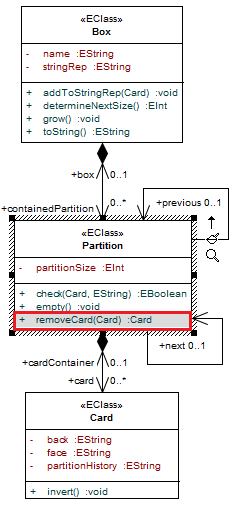
\includegraphics[width=0.4\textwidth]{pics/sdmBilder/removeCard/sdm01RAW}
  \caption{Double-click a method to implement it.}  
  \label{fig:sdm_start}
\end{center}
\end{figure}
 
If you did everything right, a new \emph{activity diagram} should be created \note{Activity Diagram} with a cute little \emph{start node} labelled with the signature of the method \note{Start Node} as depicted in Fig.~\ref{fig:sdm_skeleton}.  Inspect your project browser and note that an \texttt{SDM\_Container} has been created for the method \texttt{removeCard} to contain the diagram.  
If you're at any time unhappy with an SDM\footnote{As you might have already noticed, we use ``SDM'' interchangeably to mean our graph transformation language or a concrete transformation (a story model) used to implement a method and consisting of an activity diagram and a pattern in each story node.  
This will all be explained in detail.}, you can always delete the appropriate container in the project browser and start from scratch, following the steps described previously to create a skeleton for a new SDM.  
Also note the new \note{SDM Toolbox} toolbox \texttt{SDM} that has been automatically opened up for the diagram and placed to the left above the common toolbox. 

\begin{figure}[htp]
\begin{center}
  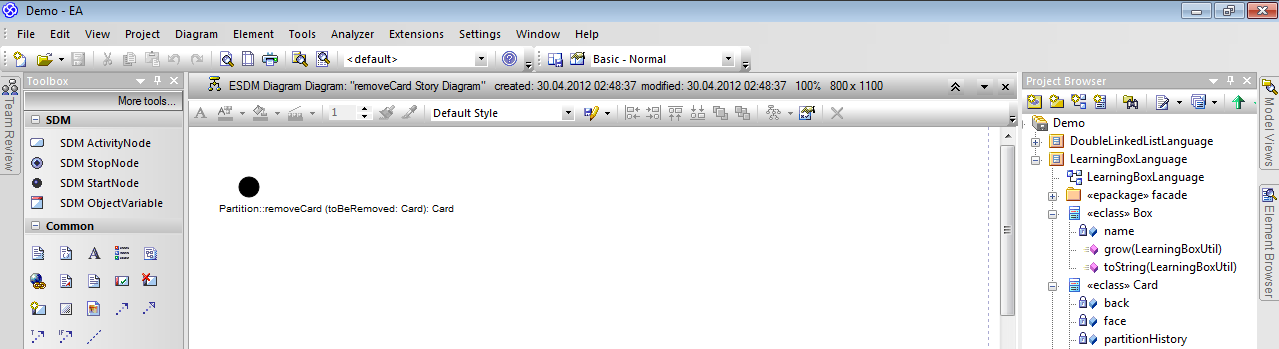
\includegraphics[width=0.9\textwidth]{pics/sdmBilder/removeCard/sdm02RAW}
  \caption{Generated SDM diagram and start node.}  
  \label{fig:sdm_skeleton}
\end{center}
\end{figure}

\subparagraph{Metamodel Validation in Eclipse:}
\label{par:validation_in_eclipse}
An activity diagram consisting of only a start node is actually not yet sufficient for any reasonable code generation. 
Nonetheless, export by choosing ``Extensions/\-MOFLON::Ecore Addin/\-Export all to Workspace'' and refresh your Eclipse project to invoke code generation. 
In Eclipse, an error dialogue should pop-up as depicted in Fig.~\ref{fig:eclipse_error}.

\begin{figure}[htp]
\begin{center}
  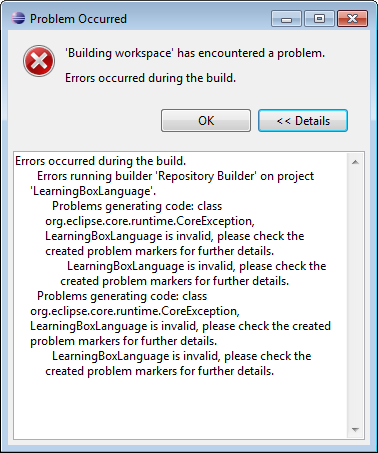
\includegraphics[width=0.4\textwidth]{pics/sdmBilder/removeCard/sdm15RAW}
  \caption{Eclipse error after generating code for invalid activity}  
  \label{fig:eclipse_error}
\end{center}
\end{figure}

This error indicates that your \texttt{Learning\-Box\-Language} was invalid and that the code generation process has failed. 
You can also see that the file \texttt{Learning\-Box\-Language.\-ecore} in the \texttt{model} folder of your project is marked as being faulty.
To see what the problem was, check the \texttt{Problems} view in Eclipse (Fig.~\ref{fig:eclipse_problems_view}), 
\note{Stop Node}
which should contain a message that an SDM must have at least one \emph{stop node} for successful code generation.

\begin{figure}[htp]
\begin{center}
  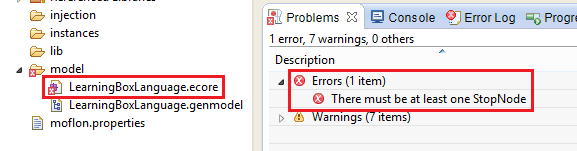
\includegraphics[width=\textwidth]{pics/sdmBilder/removeCard/sdm17RAW}
  \caption{Problems view after validation in Eclipse}  
  \label{fig:eclipse_problems_view}
\end{center}
\end{figure}

Switch back to EA and validate your metamodels again by choosing ``Extensions/MOFLON::Ecore Addin/Validate All''.
You should now see a new \texttt{Eclipse Error} in the validation output, which displays the validation results from Eclipse concerning the missing stop node of the \texttt{removeCard} activity (Fig~\ref{fig:ea_eclipse_error}). 

\begin{figure}[htp]
\begin{center}
  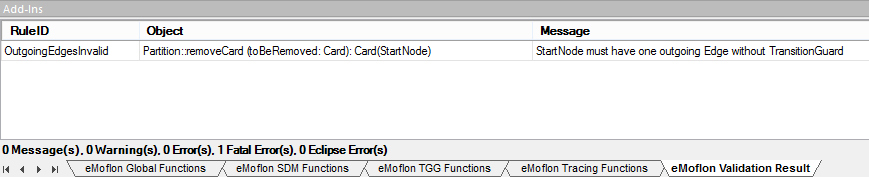
\includegraphics[width=0.6\textwidth]{pics/sdmBilder/removeCard/sdm16RAW}
  \caption{EA validation output for a start node without an outgoing edge after an Eclipse error}  
  \label{fig:ea_eclipse_error}
\end{center}
\end{figure}


Our validation mechanism checks the dynamic semantics (SDMs) of your metamodels, partly by rule checking directly in EA and by communicating with Eclipse after the code generation process. 
Please note that the corresponding error message in EA only appeared \emph{after} the validation in Eclipse and won't be deleted until the next successful code generation process in Eclipse and a subsequent validation in EA.

This means that to get rid of the error message in EA, you must (1) correct the error by completing the activity as described below, (2) export from EA, (3) successfully generate code in Eclipse and (4) validate again in EA after code generation in Eclipse.\\
\noindent\rule[-1ex]{0.5\textwidth}{0.5pt}\\

Now it's time to complete our very first activity. 
Choose the start node, and note the small black arrow that appears (Fig.~\ref{fig:sdm_quicklink}).  
Similar to quick linking which we learnt when creating our metamodel, a further fundamental gesture in EA is \emph{Quick
\note{Quick Create} 
Create}. 
To quick create an element, pull the arrow and click on an empty spot in the diagram where the new element is to be created.  
This is basically quick linking to a non-existent element if you wish.

\begin{figure}[htp]
\begin{center}
  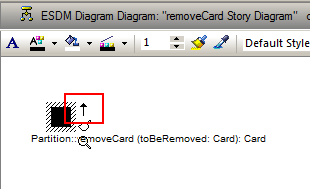
\includegraphics[width=0.5\textwidth]{pics/sdmBilder/removeCard/sdm03RAW}
  \caption{Quick link in SDM diagram to create new activity node.}  
  \label{fig:sdm_quicklink}
\end{center}
\end{figure}

EA notices that there is nothing to quick link to and pops up a small context-sensitive dialogue, not for creating a link as in the case of quick linking, but for creating an element that can be connected to the indicated source element. 

As indicated in Fig.~\ref{fig:sdm_new_activity_node} choose \texttt{Append StoryNode} to create an \emph{activity node}.  
We
\note{Activity}
\note{Activity Node}
\note{Activity Edge}
shall refer to the whole activity diagram simply as an \emph{activity} that always starts with a start node, terminates with a \emph{stop node} and consists of activity nodes connected via \emph{activity edges}.  
If you quick created correctly, you should now have a start node, an activity node called \texttt{ActivityNode 1} and an edge connecting the start node and the activity node.

\begin{figure}[htp]
\begin{center}
  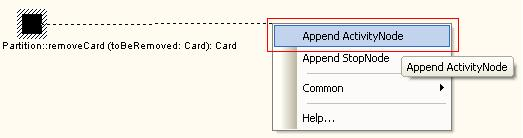
\includegraphics[width=0.8\textwidth]{pics/sdmBilder/removeCard/sdm04RAW}
  \caption{Create new activity node.}  
  \label{fig:sdm_new_activity_node}
\end{center}
\end{figure}

Complete the activity by quick creating a stop node as depicted in Fig.~\ref{fig:sdm_stop_node}.

\begin{figure}[htp]
\begin{center}
  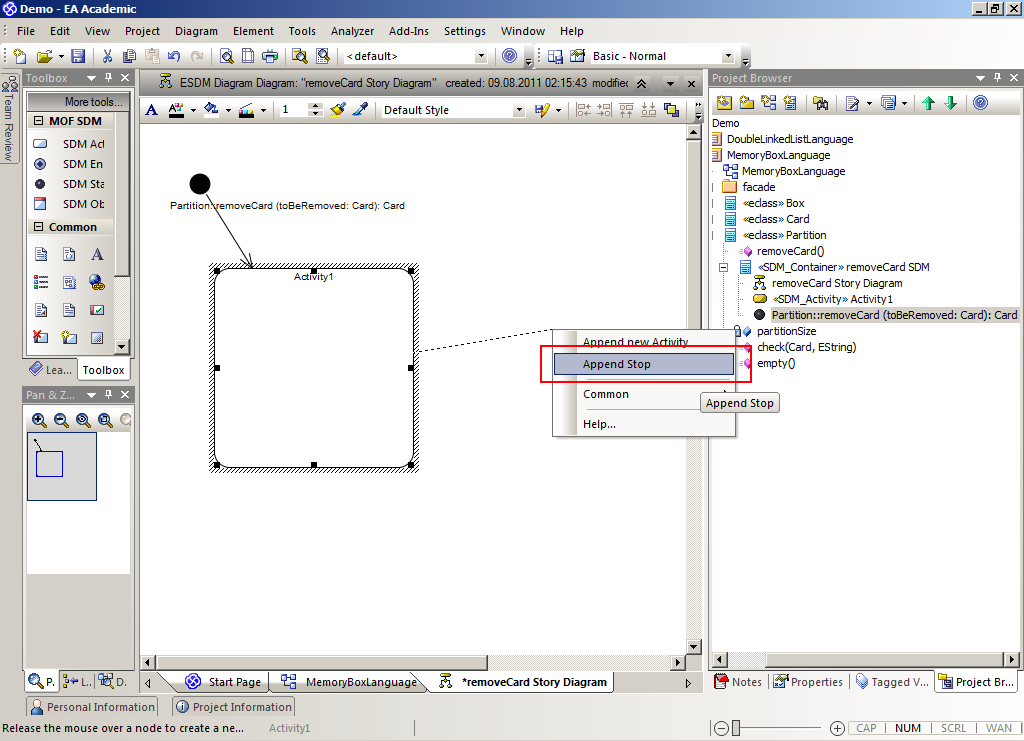
\includegraphics[width=0.8\textwidth]{pics/sdmBilder/removeCard/sdm05RAW}
  \caption{Complete activity with a stop node.}  
  \label{fig:sdm_stop_node}
\end{center}
\end{figure}

If you did that right as well you should now have a complete activity that models the procedural \emph{control flow} of our method.  
The semantics of our activities is pretty straightforward -- the control flow starts in the start node and flows along edges and connected activity nodes till it terminates in a stop node.  
The complete activity is depicted in Fig.~\ref{fig:sdm_complete_control_flow_simple} now with the activity node connected via an activity edge to the newly created stop node.

\label{story-pattern}

Integrated as an atomic step in this overall control flow, a single graph
\note{Story Pattern}
transformation step can be embedded in some activity nodes as a \emph{story pattern}.  
These story patterns are declarative transformation rules as introduced in Sec.~\ref{sec:sdm_intro}.  
As not all activity nodes can contain story
\note{Story Node}
patterns (e.g. start and stop nodes), those that can are called \emph{story nodes}. 

\begin{figure}[htp]
\begin{center}
  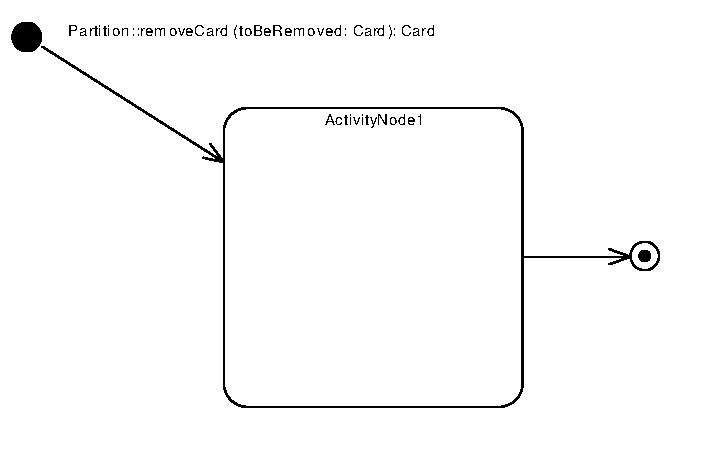
\includegraphics[width=\textwidth]{pics/sdmBilder/removeCard/sdm06RAW.pdf}
  \caption{Control flow modelled as a simple activity diagram.}  
  \label{fig:sdm_complete_control_flow_simple}
\end{center}
\end{figure}

To create a story pattern, double click the story node \texttt{ActivityNode 1} in Fig.~\ref{fig:sdm_complete_control_flow_simple} to prompt the dialogue depicted in Fig.~\ref{fig:story_pattern}.  
Enter \texttt{remove\-Card\-From\-Partition} as the name of the story node, check \texttt{Create this Object} and click \texttt{OK}.

\begin{figure}[htpb]
\begin{center} 
  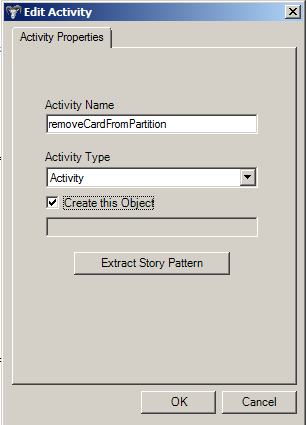
\includegraphics[width=0.45\textwidth]{pics/sdmBilder/removeCard/sdm07RAW.png}
  \caption{Start modelling story pattern in activity node.}  
  \label{fig:story_pattern}
\end{center}
\end{figure}

The activity node should now have a single \emph{object variable} \texttt{this}
\note{Object Variable}
(Fig.~\ref{fig:tool_box}). 
Object variables are, as the word ``variable'' indicates, place holders for actual objects in a model.  
During \emph{pattern matching},
\note{Pattern Matching}
actual objects in the  current model are assigned to the object variables in the pattern according to  the indicated type of the object variable and other conditions\footnote{We shall learn what conditions can be specified in a
few pages.}. 
In our case, the current story pattern consists of only one object variable, which is assigned (per convention) to \texttt{this} in Java (the object whose method is invoked).

\begin{figure}[htp]
\begin{center}
  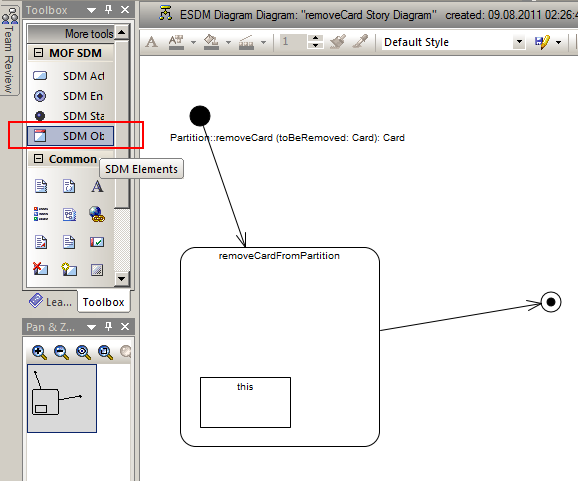
\includegraphics[width=0.8\textwidth]{pics/sdmBilder/removeCard/sdm09RAW}
  \caption{Add a new object variable from the tool-box.}  
  \label{fig:tool_box}
\end{center}
\end{figure}

To create an object variable that can be assigned to other objects, choose \texttt{SDM ObjectVariable} from the toolbox as indicated in
Fig.~\ref{fig:tool_box} and click \emph{in the} activity node \texttt{removeCardFromPartition} (Fig.~\ref{fig:object_variable_properties}). 


\begin{figure}[htp]
\begin{center}
  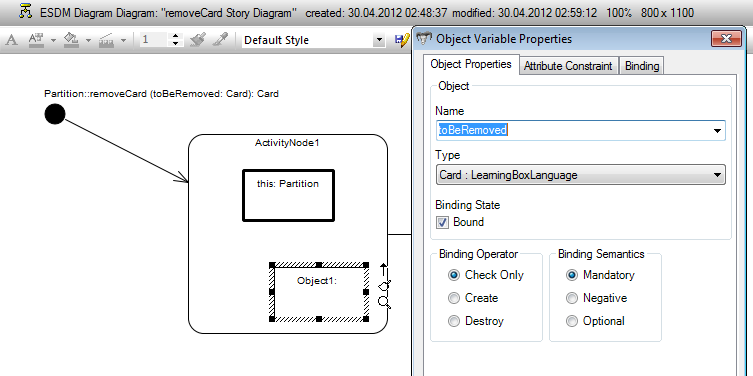
\includegraphics[width=0.8\textwidth]{pics/sdmBilder/removeCard/sdm10RAW}
  \caption{Specify properties of the added object variable.}  
  \label{fig:object_variable_properties}
\end{center}
\end{figure}

In the dialogue that pops up, choose \texttt{toBeRemoved} as the name of the object variable and \texttt{Card} as its type using the corresponding drop-down menus. 
Because \texttt{toBeRemoved} is a parameter of the method, it is offered as a possible name in the drop-down menu and can be directly chosen to prevent annoying mistakes due to typing the name of the parameter wrongly.

In the dialogue, note the option \texttt{Bound} that must be set.
For the pattern matcher, bound object variables do not need to be assigned as they already have a fixed value from the context of the method.  
We have already seen two cases  for bound object variables: the assignment to \texttt{this} (the current  partition who owns the method), and assignments to parameters of the 
\note{Binding State}
method that  are specified when invoking the method.  
Please note that the assignment or \emph{binding} is in both cases implicit and via the \emph{name} of the bound object variable. 

\begin{figure}[htp]
\begin{center}
  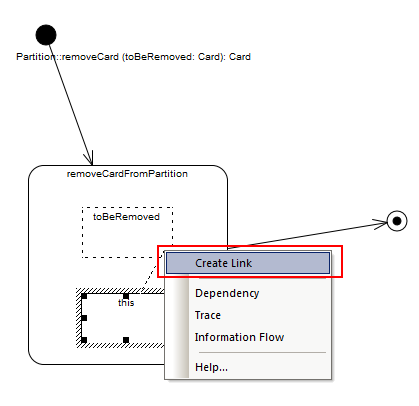
\includegraphics[width=0.6\textwidth]{pics/sdmBilder/removeCard/sdm11RAW}
  \caption{Create a link variable.}   
  \label{fig:link_variable}
\end{center}
\end{figure}

Models consist not only of objects but also of \emph{links}.  
To match links one can thus create \emph{link variables} in story patterns that act as place 
\note{Link Variable}
holders for links in a model.  
To create a link variable between the current partition, whose \texttt{removeCard} method is invoked, and the card to be removed, which is passed in as a parameter of the method, choose the object variable \texttt{this} and quick link it to the object variable \texttt{toBeRemoved}.  
In the quick link dialogue choose \texttt{Create LinkVariable} (Fig.~\ref{fig:link_variable}).

In the property dialogue that pops up, choose the offered link type (according to the metamodel, there is only one possible link type between a partition and a 
\note{Binding Operator}
card), and set the \emph{Binding Operator} to \texttt{Destroy} (Fig.~\ref{fig:link_variable_properties}). 
Every object or link variable's binding operator can be set to one of \texttt{Check Only, Create, Destroy}.

\begin{figure}[htp] 
\begin{center} 
 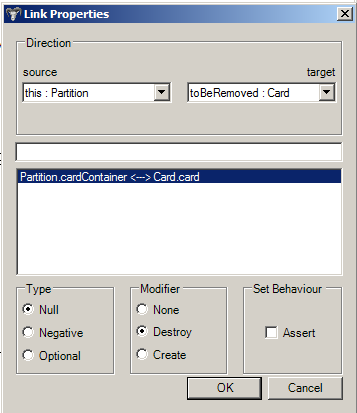
\includegraphics[width=0.6\textwidth]{pics/sdmBilder/removeCard/sdm12RAW.png}
  \caption{Specify properties for created link variable.}  
  \label{fig:link_variable_properties}
\end{center}
\end{figure}



For a rule $r: (L, R)$, as discussed in Sec.~\ref{sec:sdm_intro}, this marks the variable as belonging to the set of elements to be retained ($L\cap R$), the set of elements to be newly created ($R\setminus L$), or the set of elements to be deleted ($L\setminus R$).
 
According to the signature of the method \texttt{removeCard}, we should return the card that has been deleted.  
Although this might strike you as slightly odd, considering that we already passed in this exact card as an argument, it still makes sense as it allows for chaining method calls: \begin{quote}\texttt{aPartition.removeCard(aCard).invert()}\end{quote}
In any case, a return value for an SDM can be specified in the stop node.
\note{Return Values}
As depicted in Fig.~\ref{fig:stop_node_return_value}, double-click the stop node to prompt the \texttt{Edit StopNode} dialogue.
\note{Expressions}
In the \texttt{Expression} field, choose \texttt{ParameterExpression}, and \texttt{toBeRemoved} as the parameter.  
In many different dialogues, we employ a simple context-sensitive expression language for specifying required values.  
We have intentionally avoided creating a full-blown sub-language and limit expressions to a few simple types\footnote{We also do not support nesting expressions}.  
The philosophy here is to keep things simple and concentrate on what SDMs are good for -- expressing structural change.  
Our approach is to provide a clear and type-safe interface to a general purpose language (in our case Java) and support a simple \emph{fallback} as soon as things get low-level and difficult to express as a pattern.  

\begin{figure}[htp]
\begin{center}
  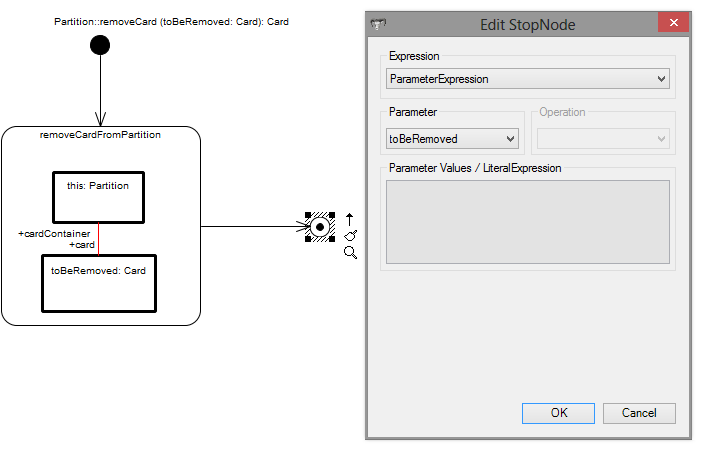
\includegraphics[width=0.95\textwidth]{pics/sdmBilder/removeCard/sdm14RAW.png}
  \caption{Adding a return value to the stop node.}  
  \label{fig:stop_node_return_value}
\end{center}
\end{figure}

The alternative approach would be to support arbitrary expressions, for example, in a script language like JavaScript or in an appropriate DSL\footnote{A DSL is a Domain Specific Language: a language designed for a specific task which is usually simpler than a general purpose language like Java and more suitable for the exact task.} designed for this purpose. 
In a few pages we'll learn the other expression types
\note{Parameter Expression}
we support and how to use them, for the moment, a \emph{Parameter Expression} is used to refer to one of the parameters of the current method, which is exactly what we needed and have used for our \texttt{removeCard} SDM.
If you've done everything right, your complete SDM should now look like Fig.~\ref{fig:sdm_complete_control_flow} with the return value indicated below the stop node.

Let's take a step back and review briefly what we have specified:  if \texttt{p.remove\-Card(c)} is invoked for a partition \texttt{p} with a card \texttt{c} as argument, the specified pattern will \emph{match} if the card is contained in the partition.
After determining a match for all variables, the link between the partition and the card is deleted, effectively ``removing'' the card from the partition.  

If the card is \emph{not} contained in the partition, the pattern won't match and nothing happens. 
In both cases the card that was passed in is simply returned.

\begin{figure}[htbp]
\begin{center}
  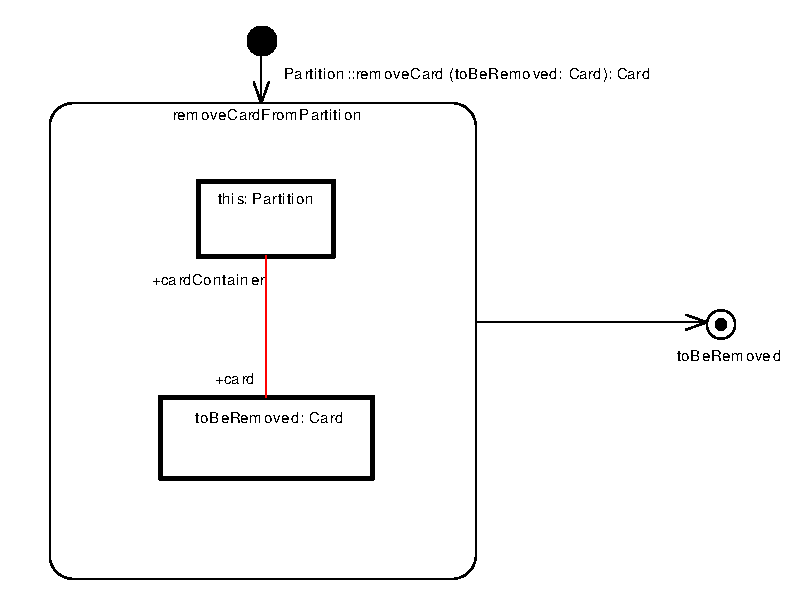
\includegraphics[width=0.95\textwidth]{pics/sdmBilder/removeCard/sdm15}
  \caption{Complete SDM for \texttt{Partition::removeCard}.}  
  \label{fig:sdm_complete_control_flow}
\end{center}
\end{figure}

Congratulations!  You have specified your very first SDM.  
Don't forget to export and generate code in your Eclipse workspace. 
Inspect the generated implementation for the method\footnote{The generated method is in \texttt{/Learning\-Box\-Language/\-gen/\-Learning\-Box\-Language/\-impl/\-Partition\-Impl.java/\-remove\-Card}} and see if you can get a feel for what the generated code does. 
Notice all the null checks that are generated automatically -- only a very conscientious (and probably slightly paranoid) programmer would program so defensively!

If you're unable to export or generate code successfully, compare your SDM carefully with Fig.~\ref{fig:sdm_complete_control_flow} and make sure you haven't forgotten anything.

In the following sections, we shall explore further features of SDM that allow for really expressive and powerful patterns.
